\documentclass[tikz,convert={outfile=\jobname.svg}]{standalone}
\begin{document}
   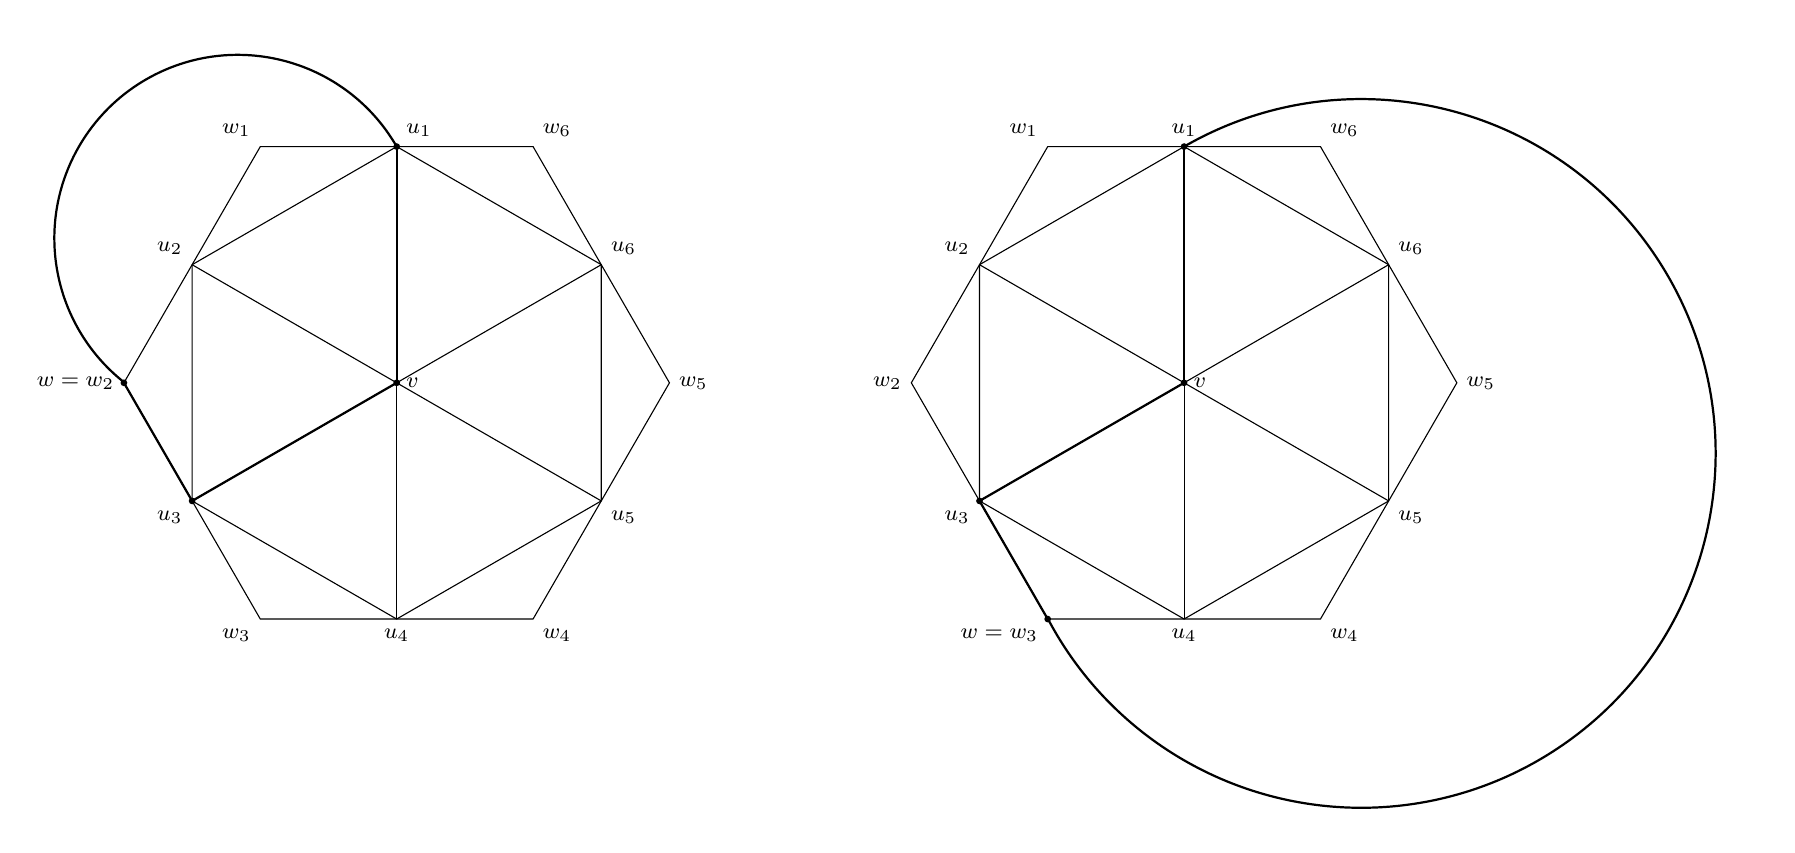
\begin{tikzpicture}
      \def\R{3cm}
      \def\RRR{3.4641cm} % R csc(60°)
      \begin{scope}
         \draw (0: 0) node[anchor=west]{\footnotesize$v$};
         \draw (0: \RRR) node[anchor=west]{\footnotesize$w_5$};
         \draw (60: \RRR) node[anchor=south west]{\footnotesize$w_6$};
         \draw (120: \RRR) node[anchor=south east]{\footnotesize$w_1$};
         \draw (180: \RRR) node[anchor=east]{\footnotesize$w = w_2$};
         \draw (240: \RRR) node[anchor=north east]{\footnotesize$w_3$};
         \draw (300: \RRR) node[anchor=north west]{\footnotesize$w_4$};
         \draw (90: \R) node[anchor=south west]{\footnotesize$u_1$};
         \draw (150: \R) node[anchor=south east]{\footnotesize$u_2$};
         \draw (210: \R) node[anchor=north east]{\footnotesize$u_3$};
         \draw (270: \R) node[anchor=north]{\footnotesize$u_4$};
         \draw (330: \R) node[anchor=north west]{\footnotesize$u_5$};
         \draw (30: \R) node[anchor=south west]{\footnotesize$u_6$};
         \draw (0: \RRR) \foreach \x in {0, 60, ..., 300} {
            -- (\x: \RRR)
         } -- cycle;
         \draw (30: \R) \foreach \x in {90, 150, ..., 330} {
            -- (\x: \R)
         } -- cycle;
         \foreach \x in {30, 90, ..., 330} {
            \draw (0: 0) -- (\x: \R);
         }
         \filldraw[black] (0: 0) circle(1pt);
         \filldraw[black] (90: \R) circle(1pt);
         \filldraw[black] (180: \RRR) circle(1pt);
         \filldraw[black] (210: \R) circle(1pt);
         \draw[thick] (0: 0) -- (90: \R);
         \draw[thick] (90: \R) arc(30: 231: 2.33);
         \draw[thick] (180: \RRR) -- (210: \R);
         \draw[thick] (210: \R) -- (0: 0);
      \end{scope}
      \begin{scope}[xshift=10cm]
         \draw (0: 0) node[anchor=west]{\footnotesize$v$};
         \draw (0: \RRR) node[anchor=west]{\footnotesize$w_5$};
         \draw (60: \RRR) node[anchor=south west]{\footnotesize$w_6$};
         \draw (120: \RRR) node[anchor=south east]{\footnotesize$w_1$};
         \draw (180: \RRR) node[anchor=east]{\footnotesize$w_2$};
         \draw (240: \RRR) node[anchor=north east]{\footnotesize$w = w_3$};
         \draw (300: \RRR) node[anchor=north west]{\footnotesize$w_4$};
         \draw (90: \R) node[anchor=south]{\footnotesize$u_1$};
         \draw (150: \R) node[anchor=south east]{\footnotesize$u_2$};
         \draw (210: \R) node[anchor=north east]{\footnotesize$u_3$};
         \draw (270: \R) node[anchor=north]{\footnotesize$u_4$};
         \draw (330: \R) node[anchor=north west]{\footnotesize$u_5$};
         \draw (30: \R) node[anchor=south west]{\footnotesize$u_6$};
         \draw (0: \RRR) \foreach \x in {0, 60, ..., 300} {
            -- (\x: \RRR)
         } -- cycle;
         \draw (30: \R) \foreach \x in {90, 150, ..., 330} {
            -- (\x: \R)
         } -- cycle;
         \foreach \x in {30, 90, ..., 330} {
            \draw (0: 0) -- (\x: \R);
         }
         \filldraw[black] (0: 0) circle(1pt);
         \filldraw[black] (90: \R) circle(1pt);
         \filldraw[black] (210: \R) circle(1pt);
         \filldraw[black] (240: \RRR) circle(1pt);
         \draw[thick] (0: 0) -- (90: \R);
         \draw[thick] (90: \R) arc(120: -152.1: 4.5);
         \draw[thick] (240: \RRR) -- (210: \R);
         \draw[thick] (210: \R) -- (0: 0);
      \end{scope}
   \end{tikzpicture}
\end{document}
